\chapter{Introduction}
\label{introduction}

\todo {\begin{itemize} 
  \item This chapter requires major revision after Chapters 2--5 have
    been drafted.
  \item Additional matter on motivating literature for cancer has to be
    added.
  \item  A comparison with modern growth papers needs to be
    added.
  \item Citations warnings need to be fixed.
\end{itemize}}

This dissertation presents a continuum treatment of growth in
biological tissue developed within the context of modern mixture
theory. The crux of this work is a careful examination of the
assumptions underlying continuum thermodynamics under the condition
that multiple interacting species occupy a region of Euclidean space
simultaneously. The formal axiomatic treatment presented derives from
these assumptions, and provides insight into the sequence of
interaction between tissue mechanics, mass transport and biochemical
reactions. A computational formulation built upon the theory is used
to solve a broad class of numerical examples demonstrating several
biophysical aspects of tissue growth.

This initial chapter serves primarily to motivate the research and
provide some context for this work (Section~\ref{background}). It also
briefly articulates the goals of this present investigation and
defines its scope (Section~\ref{goals}), before concluding with an
overview of the topics considered in the remainder of the dissertation
(Section~\ref{overview}).

\section{Background and motivation}
\label{background}

Development of biological tissue, when described in the biomechanics
literature, is generally broken down into the distinct processes of
\emph{growth}, \emph{remodelling} and \emph{morphogenesis}. Growth, or
conversely, resorption, involves the addition or loss of
mass. Remodelling results from a change in microstructure, which could
manifest itself as an evolution of macroscopic quantities such as
state of internal stress, stiffness or material symmetry. It also
appears sometimes as fibrosis or hypertrophy. Morphogenesis involves
both growth and remodelling, as well as more complex changes in
form. A classical example of morphogenesis is the development of an
embryo from a fertilised egg. These terms are based on the definitions
developed by \cite{Taber:95}, and will be followed in this work. This
dissertation focuses exclusively on growth, its continuum formulation,
and the implications that the process holds for the standard machinery
of continuum mechanics. Remodelling is treated elsewhere
\citep{remodelpaper}. And the larger, more complex problem of
morphogenesis is beyond the scope of this body of work.

The ideas here are applicable to soft (e.g., tendon, muscle) and
hard (e.g., bone) tissue. In this paper, growth of biological
tissue will be treated at a macroscopic scale. The continuum
formulation (e.g., constitutive laws) at this scale may be
motivated by cellular, sub-cellular or molecular processes.
However, we will not explicitly model processes at this fine a
scale. The formulation can be applied with a specific tissue e.g.,
muscle, as the body of interest. Our experiments, described
separately, are on self-organizing tendon \citep{Calve:04}
and cardiac muscle constructs \citep{Baaretal:2003}, engineered
{\it in vitro}.

\begin{figure}[!hpt]
\centering
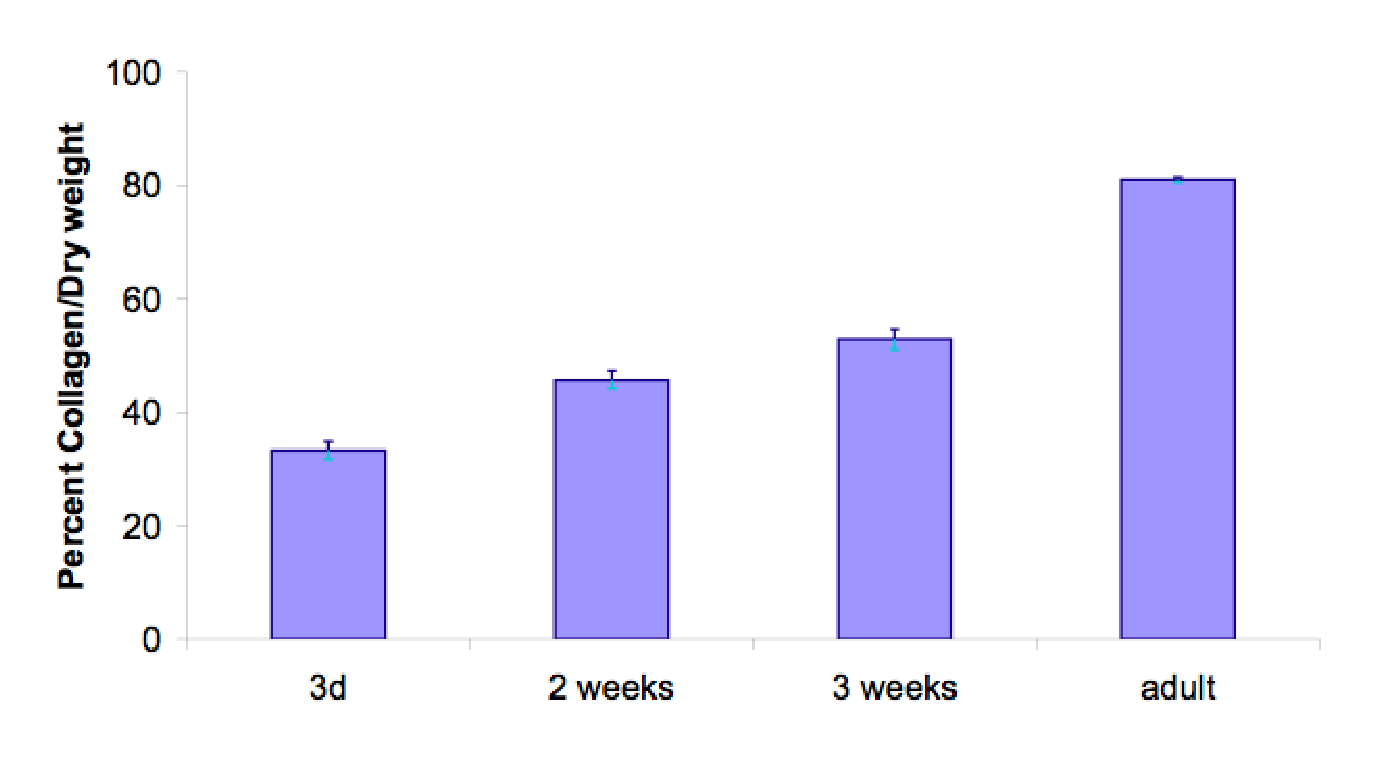
\includegraphics[width=0.8\textwidth]
                {images/experiments/content-evolution} 
\caption{Growth: An increase in collagen concentration with age.}
\label{content-evolution}
\end{figure}

The principal notion to be borne in mind while developing a
continuum formulation for growth is that one is presented with a
system that is open with respect to mass. Scalar mass sources and
sinks, and vectorial mass fluxes must be considered. A mass source
was first introduced in the context of biological growth by
\citet{CowinHegedus:76}. The mass flux is a more recent addition
of \citet{EpsteinMaugin:2000}, who, however, did not elaborate on
the specific nature of the transported species.
\citet{KuhlSteinmann:02} also incorporated the mass flux and
specified a Fickean diffusive constitutive law for it. In their
paper the diffusing species is the material of the tissue itself.
The approach to mass transport that is followed in our paper is
outlined in the next two paragraphs.

In order to be precise about the physiological relevance of our
formulation, we have found it appropriate to adopt a different
approach from the papers in the preceding paragraph in regard to
mass transport. We do not consider mass transport of the material
making up any tissue during growth. Instead, it is the nutrients,
enzymes and amino acids necessary for growth of tissue, byproducts
of metabolic reactions, and the tissue's fluid phase
\citep{Swartzetal:99} that undergo diffusion\footnote{We use the
terms ``mass transport'' and ``diffusion'' interchangeably.} in
our treatment. There do exist certain physiological processes in
which cells or the surrounding matrix migrate within a tissue. One
such process is observed when leukocytes (white blood cells) such
as neutrophils and monocytes are signalled to pass through a
capillary wall and are induced, by specific chemical attractors,
to migrate to a site of infection. This is the process of
chemotaxis \citep{GuytonHall:1996,Vander:2003}. The migrant cells
or matrix then participate in some form of cell proliferation or
death. Fibroblasts also migrate within the extra cellular matrix
during wound healing. A third example is the migration of stem
cells to different locations during the embryonic development of
an animal. These processes involve very \emph{short range}
diffusion, and can be treated by the approach described in this
paper. We have chosen to focus upon homeostasis, defined by
\citet{Vander:2003} as ``\dots a state of reasonably stable
balance betweoen the physiological
variables\dots''\footnote{\citet{Vander:2003} go on to say: ``This
simple definition cannot give a complete appreciation of what
homeostasis truly entails, however. There probably is no such
thing as a physiological variable that is constant over long
periods of time. In fact, some variables undergo fairly dramatic
swings about an average value during the course of a day, yet may
still be considered `in balance'. That is because homeostasis is a
\emph{dynamic process}, not a static one.''}. Since, to the best
of our knowledge, processes of the type just described are not
observed during homeostatic tissue growth, we will ignore
transport of the solid phase of the tissue.

The processes of cell proliferation and death, hypertrophy and
atrophy, are complex and involve several cascades of biochemical
reactions. We will treat them in an elementary fashion, using
source/sink terms that govern inter-conversion of species, and the
mass fluxes that supply reactants and remove byproducts. The
treatment will be mathematical; specific constituents will not be
identified with any greater detail than to say that they are
either the tissue's solid phase, the interstitial fluid phase,
precursors of the solid phase (these would include amino acids,
nutrients and enzymes), or byproducts of reactions. We will return
to explicitly incorporate biochemical and cellular processes
within our description of mass transport in a subsequent paper.

Virtually all biological tissue consists of a solid and fluid
phase and can be treated in the context of mixture theory
\citep{TruesdellToupin:60,TruesdellNoll:65,BedfordDrumheller:1983}.
When growth is of interest, additional species (reactants and
byproducts) must be considered as outlined above. The solid phase
is an anisotropic composite that is inhomogeneous at microscopic
and macroscopic scales. The fluid, being mostly water, may be
modelled as incompressible, or compressible with a very large bulk
modulus. This level of complexity will be maintained throughout
our treatment. The use of mixture theory leads to difficulties
associated with partitioning the boundary traction into portions
corresponding to each species. \cite{RajagopalWineman:1990},
suggested a resolution to this problem that holds in the case of
saturated media---a condition that is applicable to soft
biological tissue. An alternative is to apply the theory of porous
media that grew out of the classical work of Fick and Darcy in the
1800s \citep{Terzaghi:1943,deBoer:2000}. In this approach fluxes
are introduced for each species. Since a species that diffuses
must do so within some medium, one may think of the various
constituents diffusing through the solid phase\footnote{A more
sophisticated, and physiologically-correct, description is that
the interstitial fluid diffuses relative to the solid phase, while
precursors and byproducts of reactants diffuse with respect to the
fluid.}. This strategy has been adopted in the present work.

\begin{figure}[!hpt]
\centering
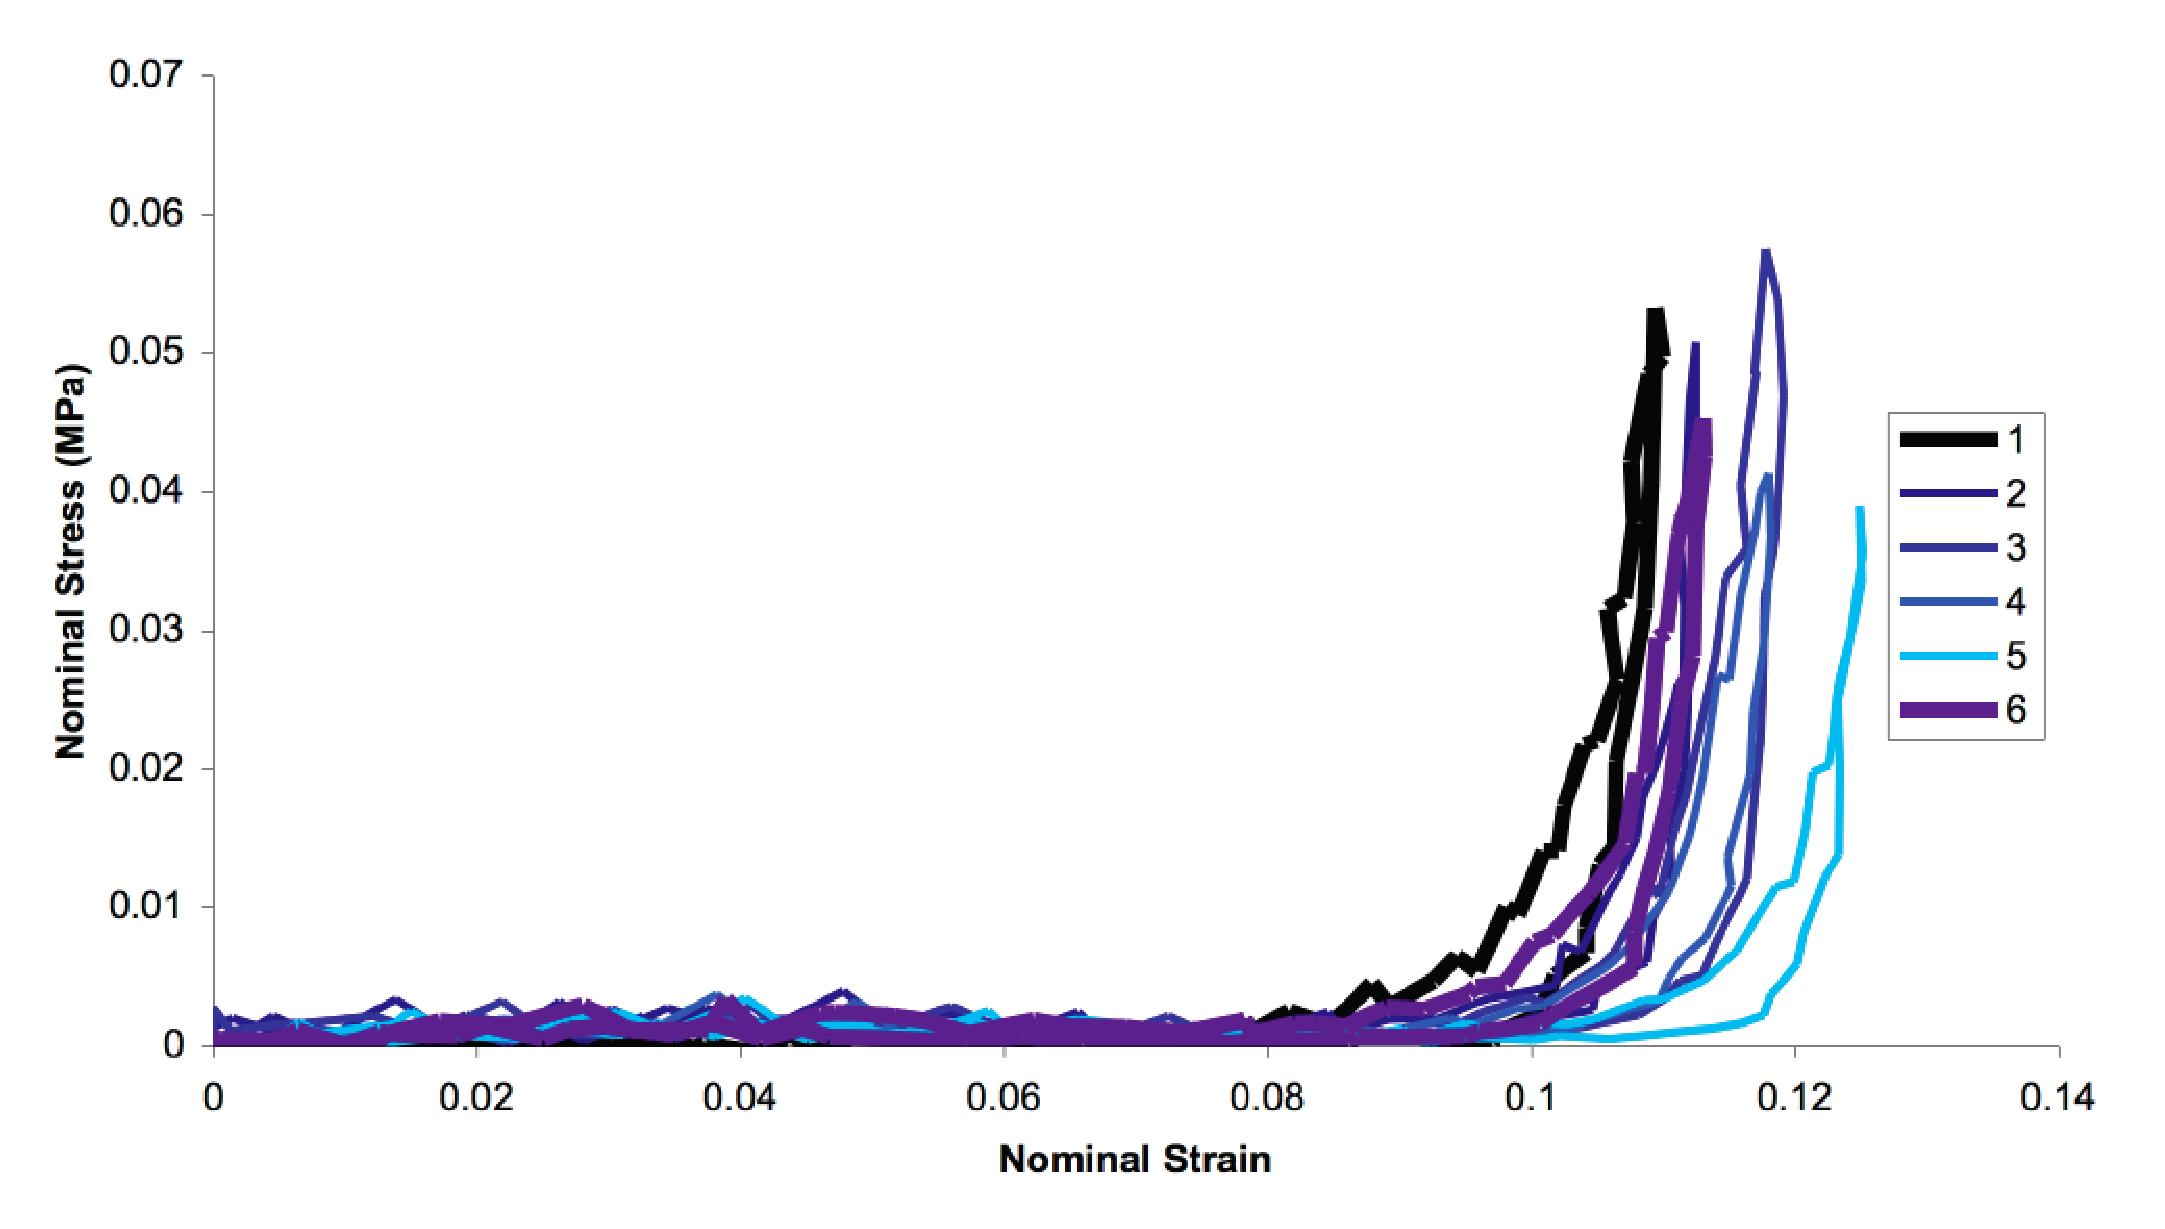
\includegraphics[width=0.8\textwidth]
                {images/experiments/tendon-cyclic-load} 
\caption{Mechanical response of a tendon under repeated cyclic loads.}
\label{tendon-cyclic-load}
\end{figure}

In a simplification that avoided the complexity of mixture theory
or porous media, \cite{CowinHegedus:76} accounted for the fluid
phase via irreversible sources and fluxes of momentum, energy and
entropy. This approach was also followed by
\cite{EpsteinMaugin:2000} and \cite{KuhlSteinmann:02}. While the
approach followed in the present paper, i.e. derivation of a mass
balance law with mass source and flux, and postulating sources and
fluxes for momentum, energy and entropy, has been attempted
recently by \cite{EpsteinMaugin:2000}, and
\cite{KuhlSteinmann:02}, there are important differences between
those works and our paper. Epstein and Maugin conclude that the
mass flux vanishes unless the internal energy depends upon strain
gradient terms (a second-order theory). This view ignores Fickean
diffusion (where the flux is linearly dependent upon concentration
of the relevant species). Our treatment also results in the
dependence of mass flux upon strain gradient, but without the
requirement of a strain gradient dependence of the internal
energy. Instead, the dissipation inequality motivates a
constitutive relation for the mass flux of each transported
species. When properly formulated in a thermodynamic setting, the
mass flux can be constrained to depend upon the strain/stress
gradient \emph{and} the gradient in concentration (mass per unit
system volume) of the corresponding species. The latter term is
the Fickean contribution to the mass flux. The form obtained is
essentially identical to \cite{DeGrootMazur:1984}.

While modelling hard biological tissue, it is common to assume a
Fickean flux, and a mass source that depends upon the strain
energy density \citep{HarriganHamilton:1993}, and therefore upon
the strain. This introduces coupling between mass transport and
mechanics. One possible difficulty with this approach is that one
could conceive of a mass source that satisfies other requirements,
such as the dissipation inequality, but does not depend upon any
mechanical quantities. Strain- or stress-mediated mass transport
would then be absent in the boundary value problems solved with
such a formulation.

\section{Goals and scope}
\label{goals}

\emph{Growth} involves the addition or depletion of mass in biological
tissue. Growth occurs in combination with
\emph{remodelling}, which is a change in microstructure, and possibly
with \emph{morphogenesis}, which is a change in form in the embryonic
state. The physics of these processes are quite distinct, and for
modelling purposes can, and must, be separated. Our previous work
\citep{growthpaper}, upon which we now seek to build, drew in some
measure from \citet{CowinHegedus:76, EpsteinMaugin:2000}, and
\citet{TaberHumphrey:2001}, and was focused upon a comprehensive
account of the coupling between transport and mechanics. The origins
of this coupling were traced to the balance equations, kinematics and
constitutive relations. A major contribution of that work was the
identification and discussion of several driving forces for transport
that are thermodynamically-consistent, in the sense that specification
of these relations does not violate the Clausius-Duhem dissipation
inequality. 

There have been a number of significant papers on biological growth
and remodelling in the last 7--8 years of which we touch upon some,
whose approaches are either similar to ours in some respects or differ
in important ways. \citet{HumphreyRajagopal:02} provided a
mathematical treatment of \emph{adaptation} in a tissue, which includes 
growth and remodelling in the sense of this paper. The authors
identified adaptation as perhaps the most important mechanical
characteristic of biological tissue. They introduced the notion of evolving
natural configurations to model the state of material deposited at
different instants in time. The treatment of the growth part of the
deformation gradient in this paper bears some resemblance to this
idea, although a detailed development has not been pursued here. The
focus, instead, is on detailing some aspects of the problem that
derive from treatment of the tissue as a porous medium, or as a
mixture of interacting species. \citet{PreziosiFarina:2002} developed an
extension to the classical Darcy's Law to incorporate mass exchanges
between reacting species. This consideration is relevant to growth
problems; however, in our opinion, these issues were subsumed in
\citet{growthpaper}, upon which this paper is based. Many of the ideas
employed here are applicable to tumour growth problems; however, due
to our current focus on tendon, we do not include phenomena
such as angiogenesis and cell migration \citep[see for
  example][]{Brewardetal:2003}. The changes in concentration that
occur with growth tend to cause swelling or contraction of the
tissue. This phenomenon has been accounted for previously by us in fields unrelated to
Biology, using the idea of thermal expansion. See, for
example, \citet{Rao2:00} and \citet{Garikipatietal:01}, which, too,
are probably not the first instances of this idea. In the literature
on biological 
growth this connection was made by \citet{KlischHoger:2003}.

In the present paper, we seek to restrict the range of
physically-admissible models in order to gain greater
physiological relevance for modelling growth in soft biological
tissue. We also include one improvement in the mathematical/numerical treatment:
The advection-diffusion equations for mass transport
require numerical stabilisation in the advection-dominated regime
(the hyperbolic limit). We draw upon the enforcement of the
incompressibility limit for the fluid phase to facilitate this
development. Below, we briefly introduce each aspect that we have
considered, but postpone details until relevant sections in the paper.

\begin{itemize}
\item[\textbullet] For a tissue undergoing finite strain, the
  transport equations can be formulated, mathematically, in terms of
  concentrations with respect to either the reference or current
  (deformed) configuration. However, the physics of fluid-tissue
  interactions and the imposition of relevant boundary conditions is
  best understood and represented in the current configuration.

\item[\textbullet] The state of saturation is crucial in determining
  whether the tissue swells or shrinks with infusion/expulsion of
  fluid. This aspect has been introduced into the formulation.

\item[\textbullet] The fluid phase, whether slightly compressible or
  incompressible, can develop compressive stress without
  bound. However, it can develop at most a small tensile stress
  \citep{cavitationchris}, having implications for the stiffness of
  the tissue in tension as against compression. Although 
  this also has implications for void formation through cavitation,
  the ambient pressure in the tissue under normal physiological
  conditions ensures that this manifests itself only as a reduction in
  compressive pressure.

\item[\textbullet] When modelling transport, it is common to assume
  Fickean diffusion \citep{KuhlSteinmann:02}. This implies the
  existence of a mixing entropy due to the configurations available to
  molecules of the diffusing species at fixed values of the
  macroscopic concentration. The state of fluid saturation directly
  influences its mixing entropy.

\item[\textbullet] If fluid saturation is maintained, void formation
  in the pores is disallowed even under an increase in the pores'
  volume. This has implications for the fluid exchanges between a
  deforming tissue and a fluid bath with which it is in contact.

\item[\textbullet] Recognising the incompressibility of the fluid
  phase, it is common to treat soft biological tissue as either
  incompressible or nearly-incompressible \citep{Fung:1993}. At the
  scale of the pores (the microscopic scale in this case), however, a
  distinction exists in that the fluid is exactly (or nearly)
  incompressible, while the porous solid network is not obviously
  incompressible.

\item[\textbullet] In \citet{growthpaper}, the acceleration of the
  solid phase was included as a driving force in the constitutive
  relation for the flux of other phases. However, acceleration is not
  frame-invariant and its use in constitutive relations is
  inappropriate.

\item[\textbullet] Chemical solutes in the extra-cellular fluid are
  advected by the fluid velocity and additionally undergo transport
  under a chemical potential gradient relative to the fluid. In the
  hyperbolic limit, where advection dominates, spatial instabilities
  emerge in numerical solutions of these transport equations
  \citep{Brooks:82, Paper6}. Numerical stabilisation of the equations
  is intimately tied to the mathematical representation of fluid
  incompressibility.

\item[\textbullet] The modelling of solid-fluid mechanical coupling
  carries strong implications for the stiffness of tissue response,
  the nature of fluid transport, and since nutrients are dissolved in
  the fluid, ultimately for growth. We present upper and lower bounds
  for this problem and computations of coupled boundary value problems with
  these bounds.
\end{itemize}

\section{Overview}
\label{overview}

The present paper is aimed at a complete treatment of mass
transport, coupled with mechanics, for the growth problem. Initial
sections (Sections \ref{sect2}--\ref{sect3bis}) treat the balance
of mass, balance of linear and angular momenta, the forms of the
First and Second Laws for this problem, and kinematics of growth,
respectively. The Clausius-Duhem inequality and its implications
for constitutive relations are the subject of Section \ref{sect5}.
Examples are provided as appropriate to illustrate the important
results. A preliminary numerical example appears in Section
\ref{sect6}. A discussion and conclusion are provided in Section
\ref{sect7}.

These issues are treated in detail in relevant sections of the paper,
which is laid out as follows: Balance equations and kinematics are
discussed in Section~\ref{sec:2}, constitutive relations for
reactions, transport and mechanics in Section \ref{sec:3}, and
numerical examples are presented in Section
\ref{numericalimplementation}. Conclusions are drawn in
Section~\ref{sec:5}.

%

% Local Variables:
% TeX-master: "thesis"
% mode: latex
% mode: flyspell
% End:
